% !TEX TS-program = pdflatex
% !TEX encoding = UTF-8 Unicode

% This is a simple template for a LaTeX document using the "article" class.
% See "book", "report", "letter" for other types of document.

\documentclass[11pt]{article} % use larger type; default would be 10pt

\usepackage[utf8]{inputenc} % set input encoding (not needed with XeLaTeX)

%%% Examples of Article customizations
% These packages are optional, depending whether you want the features they provide.
% See the LaTeX Companion or other references for full information.

%%% PAGE DIMENSIONS
\usepackage{geometry} % to change the page dimensions
\geometry{a4paper} % or letterpaper (US) or a5paper or....
% \geometry{margin=2in} % for example, change the margins to 2 inches all round
% \geometry{landscape} % set up the page for landscape
%   read geometry.pdf for detailed page layout information

\usepackage{graphicx} % support the \includegraphics command and options

% \usepackage[parfill]{parskip} % Activate to begin paragraphs with an empty line rather than an indent

%%% PACKAGES
\usepackage{booktabs} % for much better looking tables
\usepackage{array} % for better arrays (eg matrices) in maths
\usepackage{paralist} % very flexible & customisable lists (eg. enumerate/itemize, etc.)
\usepackage{verbatim} % adds environment for commenting out blocks of text & for better verbatim
\usepackage{subfig} % make it possible to include more than one captioned figure/table in a single float
\usepackage{amsmath} 
% These packages are all incorporated in the memoir class to one degree or another...

%%% HEADERS & FOOTERS
\usepackage{fancyhdr} % This should be set AFTER setting up the page geometry
\pagestyle{fancy} % options: empty , plain , fancy
\renewcommand{\headrulewidth}{0pt} % customise the layout...
\lhead{}\chead{}\rhead{}
\lfoot{}\cfoot{\thepage}\rfoot{}

%%% SECTION TITLE APPEARANCE
\usepackage{sectsty}
\allsectionsfont{\sffamily\mdseries\upshape} % (See the fntguide.pdf for font help)
% (This matches ConTeXt defaults)

%%% ToC (table of contents) APPEARANCE
\usepackage[nottoc,notlof,notlot]{tocbibind} % Put the bibliography in the ToC
\usepackage[titles,subfigure]{tocloft} % Alter the style of the Table of Contents
\renewcommand{\cftsecfont}{\rmfamily\mdseries\upshape}
\renewcommand{\cftsecpagefont}{\rmfamily\mdseries\upshape} % No bold!

%%% END Article customizations

%%% The "real" document content comes below...

\title{N-Body problem}
\author{Marcel Boersma\\Shabaz Sultan}
%\date{} % Activate to display a given date or no date (if empty),
         % otherwise the current date is printed 

\begin{document}
\maketitle

\section{Introduction}
Commonly used technology in everyday life is supported by satellites, e.g. GPS in car navigation, Internet and pictures from Google Maps. 
And with increasingly more satellites orbiting the earth it is important that we know that a new satellite will not crash into another.
Or, in more general terms we need to know how objects orbiting other objects work such that we can launch more satellites.

Although, it is not a new problem, because we have been trying to analyze how planets orbit each other in our own solar system for quite while, there is still room for improvement.
The analytical solution for orbiting planets are only purposed for 2-body system, while in reality we have to cope with N-body systems. Approximation methods can be used only calculating is intractable by hand. Hence, the use of computers is promising for solving N-body systems. However, using computers and approximation methods comes with different types of problems, i.e. how accurate is my approximation method as well as the physical limitations of computers in terms of floating point operations.

This research is aims to provide insight in the approximation methods used for N-body systems, i.e. how accurate is the simulation. 
In section~\ref{sec:literature} the background of the analytical models used are explained and section~\ref{sec:methodology} introduces the algorithms as well a methods for benchmarking our approximation methods. The results are shown in section~\ref{sec:results} and section~\ref{sec:conclusion} our conclusion is discussed.

\section{Background}
\label{sec:literature}
In pursuance of calculating the trajectory of a body it is necessary to know which forces interact with our body. Newton's seconds law, i.e. the rate of change is equal to the net force on a object, is used to describe the force on our object. And Newton's third law, i.e. action = - reaction, is used. 

\subsection{Newton's laws}
Newton's second law describes that the force on an object is equal to the change of momentum in time. Because we only consider constant mass systems this is equal to the mass times the acceleration of an object. Thus, if the object is accelerating there is a force on our object present. Knowing that the only possible object acting on our object are the other planets in the system we can modify the second law to derive the law of universal gravitation. Let the following equation be the force $F_p$ on object $p$ by object $c$ with mass $m_p,m_c$ respectively.   
\begin{equation}
    \label{eq:newtongravity}
 F_p = G\frac{m_pm_c}{r^2}
\end{equation}
With $r$ as the euclidean distance between object $p,c$. Combining Newton's second law with the law of universal gravitation gives the acceleration $a_p$ of object $p$
\begin{equation}
    \label{eq:newtongravity}
	a_p = G\frac{m_pm_c}{ m_pr^2}
\end{equation}.
The third law states that if there is a force $F_1$ then there also exists a force $F_2$ such that $F_2 = - F_1$. 

In the next section a simple 2-body system is introduced for thorough understanding the approximation methods used in later sections.


\section{Methodology}
\label{sec:methodology}
To understand the consequences of our approximation methods we first need to understand the analytical solution of a 2-body system. Next, we assume a simple two body system with an analytical solution and we will apply Newton's law to obtain the trajectory of our objects. Remark that this is special simple case designed to provided better understanding of orbiting objects, this is required to understand the effects of discrete approximation methods in our simulations. \\
\indent Assume we have a 2 body system called Pluto-Charon system. Figure~\ref{fig:plutocharon} illustrates this system at a fixed time point $t$
\begin{figure*}
	\label{fig:plutocharon}
\end{figure*}
with both $x,y$ coordinates in our 2D space.

% Assume that we have an initial velocity vector $\overrightarrow{v_t}$ for the body t with speed in both x and y direction.
% \begin{equation}
% 	\overrightarrow{v_t} = \begin{bmatrix}
% 								x_t \\
% 								y_t
% 							\end{bmatrix}
% \end{equation}
% For example we have a two body system with $p,c$ with an initial velocity vector, respectively, then
% \begin{equation}
% 	v_p=\begin{bmatrix} v_x^p \\ v_y^p \end{bmatrix}, v_c=\begin{bmatrix} v_x^c \\ v_y^c \end{bmatrix}
% \end{equation}
We assume that the whole system has a constant velocity, in our case we assume zero velocity, hence the next equation must be equal to zero
\begin{equation}
	V = \frac{P}{M}	
\end{equation}
with $P$ as the total momentum and $M$ as the total mass of the system. We know that the total momentum is the sum of all forces acted up on and the mass is a constant. Therefore, our zero velocity implies that the total momentum must be equal to zero. Or more formally
\begin{equation}
	P = m_p\overrightarrow{v_p} + m_c\overrightarrow{v_c} = 0.
\end{equation}
As illustrated in figure~\ref{XXXX}(simple two body system with vectors drawn) we can see that each body has several forces acted upon. Our objective is the determine the path of body $p,c$ and as you can see we have a force vector $F_x$ pulling the body $X$ to the center and also our velocity vector $v_x$. The product of those vectors gives us the directional vector of our body $X$. Due to the fact that the two bodies are the only objects in the system acting on each other we can determine the radius and period of our movement around a (virtual) center of mass. We know for a fact that the two bodies must be the opposites of each other such that the total momentum is equal to zero. The center of mass can be calculated in reference of one of our bodies.  (Bary center)
\begin{equation}
	(m_p + m_c)\overrightarrow{r_{m}} = m_p\overrightarrow{r_p} + m_c\overrightarrow{r_c} 
\end{equation}
With $r_m$ being the vector to the center of mass, the we can rewrite this to calculate $r_m$
\begin{equation}
	\overrightarrow{r_m} = \frac{m_p\overrightarrow{r_p} + m_c\overrightarrow{r_c}}{(m_p + m_c)}
\end{equation}
and we will calculate the $\overrightarrow{r_m}$ with as reference point our body $C$, then the $\overrightarrow{r_c}=0$ because the distance between our body $C$ and $C$ is zero, and the $\overrightarrow{r_p}=R$ with $R$ as the total distance between the two bodies. Then $\overrightarrow{r_m}$ becomes
\begin{equation}
	\overrightarrow{r_m} = \frac{m_p}{M}\overrightarrow{R}
\end{equation}


If we want to know the force of body $p$ on body $c$ we can use Newton's law of gravitation, see equation~\ref{eq:newtongravity}.  We can fill in the masses of bodies $p,c$ using the fact that $F_c = m_c a_c$ we obtain
\begin{equation}
    \begin{split}
     a_c m_c = G\frac{m_c m_p}{r^2} \\
     a_c = G\frac{m_p}{r^2} \\
    \end{split}
\end{equation}
Now that we have derived the acceleration in terms of the mass of $p$ and the distance between the bodies $r$, we can use this calculate the acceleration of body $c$. The change of position i.e. distance of body $c$ at time $\delta t$ is given by
\begin{equation}
    \frac{d^2}{dt^2} r_c = G \frac{m_p}{r^2}
\end{equation}
So the new position can be derived by taking the position at time $t=0$ plus the distance traveled during $\delta t$. This can be obtained by taking the double integral of the acceleration. This can be solved analytically when only considering two bodies. If you consider $n \geq 3$ bodies it becomes unsolvable analytically. 
\subsection{Discrete Approximation}
The N-body system for more than 2 bodies can not be solved analytically, hence we must use approximation methods to calculate the solution.
We want to obtain the new positions of our bodies at time $t+1$ by using Newton's second law. We can derive the next position by adding the distance traveled in time $\Delta t$ to the old position at $x_t$, i.e. $x_{t+1} = x_t + v_t*\Delta t$ with $v_t$ as the speed at time $t$. Nonetheless, we do not know speed $v_t$ but this can be obtained by $v_t = v_t + a_t \Delta t$ and $a_t$ is known for our body. The next section describes an even more accurate approach for $x_t$.

\subsubsection{Taylor expansion}
If we want to approximate the values of, for example, formula $f(x)$ at point $a$ we can use a Taylor expansion defined as
\begin{equation}
    \label{eq:taylor}
    \sum^\infty_{n=0} \frac{f^{(n)}(a)}{n!}(x-a)^n
\end{equation}
when we sum to infinity the new function will be the same as the original function $f(x)$. In our case we want to approximate the formulas $x(t), v(t), a(t)$ at points near $t$ and we can use equation~\ref{eq:taylor} to describe $x(t)$ as with 
\begin{equation}
    x(t) = \sum^\infty_{n=0} \frac{x^{(n)}(t)}{n!}(x-t)^n
\end{equation}
however, we are dealing with limited precision and will only use a few terms of the summation such that $x(t)$ becomes
\begin{equation}
    x(t) =  \frac{x^{(0)}(t)}{0!}(x-t)^0 + \frac{x^{(1)}(t)}{1!}(x-t)^1 +\frac{x^{(2)}(t)}{2!}(x-t)^2 +\frac{x^{(3)}(t)}{3!}(x-t)^3
\end{equation}
notice that $x^{(1)}(t)$ is the derivative of $x(t)$ which is equal to the velocity $v(t)$ and $x^{(2)}$ is equal to the acceleration $a(t)$. But we can also formulate a Taylor expansion for $v(t)$ and $a(t)$
\begin{equation}
    \begin{split}
        v(t) =  \frac{v^{(0)}(t)}{0!}(x-t)^0 + \frac{v^{(1)}(t)}{1!}(x-t)^1 +\frac{v^{(2)}(t)}{2!}(x-t)^2\\
        v(t) = v(0) + a(t) + j(t)
    \end{split}
\end{equation}
\begin{equation}
    \begin{split}
        a(t) =  \frac{a^{(0)}(t)}{0!}(x-t)^0 + \frac{a^{(1)}(t)}{1!}(x-t)^1 \\
        a(t) =  a(0) + j(t) 
    \end{split}
\end{equation}
we can calculate $j(t)$ by taking the derivative of equation~\ref{eq:newtongravity} with respect to $a$. Thus obtaining more accurate results for our $x(t), v(t)$ and $a(t)$.
Also, error of the approximation can be calculated as follows:


\subsubsection{Sensitivity analysis}
because we use approximations we have sensitive systems etc....
perturbations in input variables and output variables. i.e. positions of other objects are incorrect.
Delta step influences sensitivity?....


\subsubsection{Model verification}
\label{verification}
To verify the accuracy of the simulation we can apply some fundamental conservation laws from physics to our simulation. We know based on empirical data that these laws seem to be true for the natural, so if our simulation is a faithful model of nature these laws should also be true for our simulation. If they do not, the amount our simulation fails to conserve certain values that are supposed to be conserved can be used as a metric for the error in our simulation.\\\\
\textbf{Conservation of Momentum}\\
Momentum is defined as the mass of an object multiplied with its velocity vector. To get the momentum of a system of n bodies you can calculate the momentum of each body and sum them all together.
\begin{equation}
    \vec{p}_{total} = \sum_{i=1}^n m_i \times \vec{v_i}
\end{equation}
As long as two interacting bodies experience equal but opposite forces the conservation of momentum tends to be pretty well preserved, even if those forces are otherwise wildly inaccurate in a simulation. On the one hand this means that a fundamental law is enforced with any algorithm that ends up with the same force with a body to body interaction for both bodies, with only the direction reversed for one of them. This will be true for the n-body algorithms covered in this paper. On the other this means that the conservation of momentum is not a useful error metric to check the accuracy of an algorithm. Hence it is not used in this paper to compare the accuracy of the studied algorithms. The measurements have been done, but show no real difference, even when it is clear that a simulation is doing things that are otherwise unrealistic and inaccurate.\\\\
\textbf{Conservation of Energy}\\
Energy can not be created or destroyed, which in physics is expressed in the law of conservation of energy. Energy can be converted to a different type of energy, but the total amount of energy needs to be preserved. In a system of moving point masses that only gravitationally interact (i.e. a n-body system) the energy in the system is the sum of the kinetic energies and potential energies of each of the masses in the system. This sum should remain constant in a system that has no energy added or otherwise taken away from it. \\\\
The kinetic energy of a body is the energy it has due to its motion. The total kinetic energy of a system is the kinetic energies of all its bodies summed together.
\begin{equation}
    K = \frac{1}{2} \sum_{i=1}^n m_i |\vec{v_i}|^2
\end{equation}
The potential energy of a body is the amount of energy it experiences due to its interaction with a force field, which would be with the gravitational field in a n-body simulation. The total potential energy of a system is the sum of the potential energy of all the bodies in the system.
\begin{equation}
    W = -\frac{1}{2} \sum_{i=1, i \neq j}^n G \frac{m_i m_j}{|r_i - r_j|}
\end{equation}
The total (mechanical) energy of system is the potential and kinetic energy of the system added together, $E = W+K$. This total energy should remain constant. In a simulation this can however go wrong. For instance a body may experience a certain strong potential energy. In reality it would only experience this energy for a very short time. But in a simulation with discrete timesteps, the timestep may be longer than the time the body is supposed to experience the potential energy for. Thus it will create extra kinetic energy without that energy being based on potential energy that would be there in reality when it interact continuously with bodies rather than at discrete timesteps. \\
At the start of a simulation the initial energy in the system can be calculated. While running the simulation the energy can be calculated again. It should match the starting energy. The difference with the starting energy is the absolute energy error, and the difference divided by the current energy is the relative energy error.
\begin{equation}
    E_{error} = \frac{E_{current} - E_{initial}}{E_{current}}
\end{equation}
This relative energy error metric can be used to see how the size of the error progresses during a simulation with a particular algorithm and how the accuracy of one algorithm compares with an other algorithm.
\subsection{Algorithms}
The n-body problem involves every body in a system interacting with every other body through gravity. This means that there are $\mathcal{O}(n^2)$ interactions that need to be calculated. Very broadly n-body simulators fall into two categories. The first category contains direct solvers, which simulate the gravitational interactions between all bodies directly, e.g. phiGRAPE \cite{Harfst2007357}. \\
Alternatively, there are solvers that use a tree to represent the set of bodies in a hierarchical manner. These algorithms have each of the bodies interact with the tree instead of the full set of n-bodies. This can lead to a computational complexity of $\mathcal{O}(n \log(n))$. The Barnes-Hut algorithm is a pioneering example of this class of n-body simulation algorithms \cite{barnes1986hierarchical}.\\
We have opted to go for a direct simulator, because the implementation of such algorithms tends to be less complex. The important part in these simulations is the determination of the force each of the bodies experiences. In direct solvers, this is done the same for each body to body interactions and the total force on a particular body is a simple summation of the forces it experiences from every other body. \\
To determine the force between two bodies due to gravity is a second order differential equation needs to be solved. Thus numerical integrators are the key component of direct solvers.
\subsubsection{Integrator Algorithms}
\textbf{Euler's Method}\\
The integrators need to solve a second order differential equation. Based on calculating the force at a current point in time acceleration for a body can be determined. Based on this acceleration the position can be updated. The most straightforward way to do this is to apply Euler's method. Based on an acceleration and a stepsize $\Delta t$ it linearly approximates the speed at time $t + \Delta t$ from the speed at time $t$. Using the speed it then updates the position at time $t+\Delta t$ by linearly extrapolating from position at time $t$.
\begin{equation}
    \begin{split}
    x(t+ \Delta t) = x(t) + v(t) \Delta t \\
    v(t+ \Delta t) = v(t) + a(t) \Delta t \\
    \end{split}
\end{equation}
This integrator is appealing for its simplicity, but because it is essentially a first order taylor expansion the expected error is proportional to $\Delta t^2$.
\subsection{Implementation}
attachment
\section{Experimental Results}
\label{sec:results}
The results of each model implementation are compared using the metrics designed in section~\ref{verification}. Using these methods allows us to compare the performance of each model. For all the energy comparison methods we used a fixed total \textit{model evaluation time}, i.e. we simulate 100 model minutes. Depending on the time-steps used in each method, this might take more or less iterations to calculate, meaning that the total simulation time increases. In
section~\ref{sec:res:euler} compares the relative error of the Euler method using different time-steps. Also, section~\ref{sec:res:taylor} compares the improvement of adding an extra term in the Taylor expansion. And, section~\ref{sec:res:leapfrog} shows the results using the Leapfrog integrator and all the models are compared in the last section~\ref{sec:res:all}.

\subsection{Euler}
\label{sec:res:euler}
To verify our model, we have defined the energy metrics. In this experiment the relative energy metric as defined in section~\ref{XXX} is used. In total we have compared four different time-steps to evaluate the performance effect of an increasing/decreasing time-step. The time-steps used are $0.001, 0.01, 0.1, 1$ and figure~\ref{fig:euler} shows a plot of the relative energy error for the \textit{model simulation time}. 
\begin{figure}
    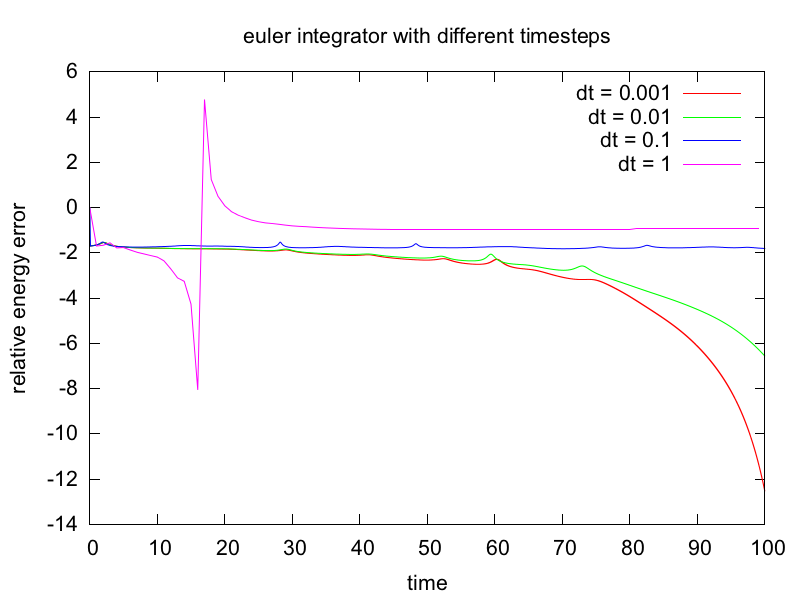
\includegraphics[width=0.9\textwidth]{euler_different_timesteps.png}
    \caption{Relative energy error for the Euler integrator using different time-steps for a fixed total model simulation time.}
    \label{fig:euler}
\end{figure}
As can be seen in figure~\ref{fig:euler} there is a spike around time 18 for time-step scale 1. This error has no apparent reason and in future time-steps it will decrease and stabilize around -1. Furthermore, it is interesting to see that with smaller time-step scales the total relative energy error increases faster. Meaning, that if we run the model for an infinite time the total error will explode and produce no meaning full results. This, while smaller time-step scales should increase the accuracy in terms of relative energy error. Therefore, we can conclude that the increase in accuracy does not outweighs the increase in iterations to complete the calculation. 

\subsection{Taylor}
\label{sec:res:taylor}
Using the same energy metrics defined in section~\ref{XX} we can do the same simulation for the Taylor approximation. We expect that adding an extra term in the Taylor expansion would increase our accuracy. And in figure~\ref{fig:taylor} we can see that indeed slower increase in relative energy error than using bigger time-step scales. However, all the time-step scale converge to -1 after about 20\% of the total model simulation time. Also, we noticed that the 0.001 time-step scale converges faster to the -1 relative energy error than the 0.0001 time-step scale. Here, we can observe that decreasing the time-step by 10 does not increase the accuracy enough to compensate for the increase in number of iterations. The could be due to machine-precision, but requires further investigation to be sure.

\begin{figure}
    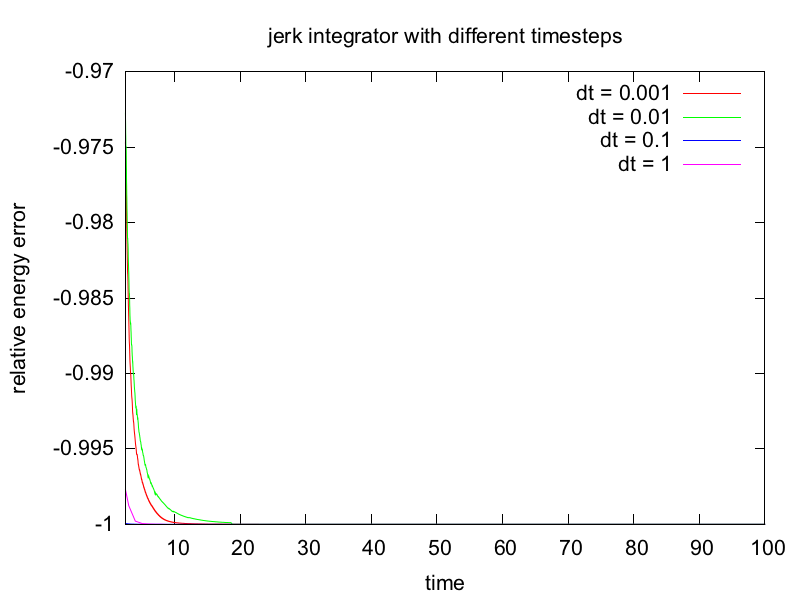
\includegraphics[width=0.9\textwidth]{jerk_different_timesteps_truncated.png}
    \caption{Relative energy error for the Taylor integrator using different time-steps for a fixed total model simulation time.}
    \label{fig:taylor}
\end{figure}

\subsection{Leapfrog}
\label{sec:res:leapfrog}
Using the Leapfrog integrator, which is a slight modified Euler integrator, we should expect similar results. And as can be seen in figure~\ref{fig:leapfrog}. the relative energy error shows similar results as for the Euler approximation in figure~\ref{fig:euler}. However, the magnitude of the relative energy error is higher with the Leapfrog integrator at around time-step 18. This is probably due to the approximation of the in between time-steps which the Leapfrog integrator uses. Nevertheless, the results are relatively the same as the Euler approximation and does, at least in our simulation, lead to a decrease in relative energy error.

\begin{figure}
    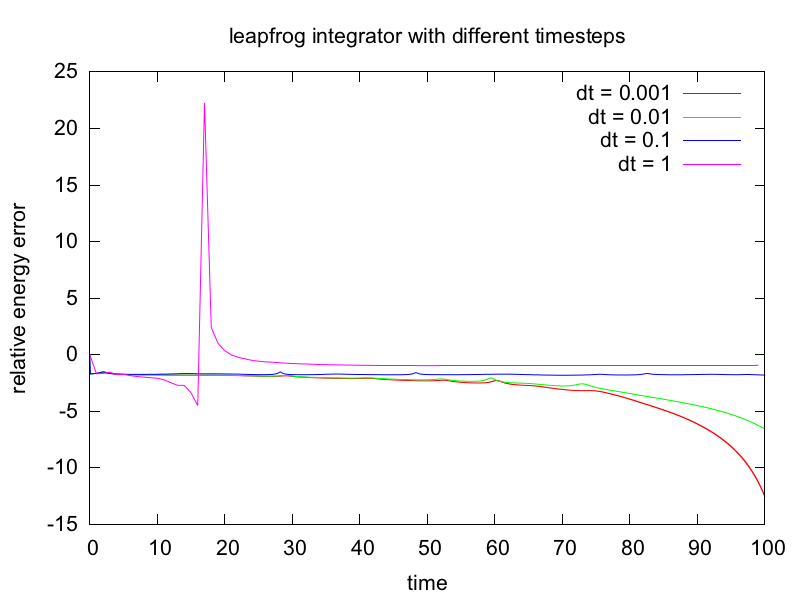
\includegraphics[width=0.9\textwidth]{leapfrog_different_timesteps.png}
    \caption{Relative energy error for the Leapfrog integrator using different time-steps for a fixed total model simulation time.}
    \label{fig:leapfrog}
\end{figure}

\subsection{Dynamic time-scales}
Each of the models is also run with the dynamic time-scale, which calculates the global minimum time-step scale such that any two bodies can not ghost through one another. However, our experiments showed that after just a few iterations the dynamic time-scale converges to the minimum allowed time-step scale by our system. Hence, it is not useful to use the dynamic time-scales in the simulations.

\subsection{All models}
\label{sec:res:all}
To compare all the models, i.e. Euler, Taylor and Leapfrog integrator, we setup up an experiment which uses the same time-step for all the models. The time-step is set at $0.01$ and figure~\ref{} shows the relative energy error for all models. Here we can clearly observe that the Taylor integrator gives the best results in terms of relative energy error. And as expected the Leapfrog and Euler integrator are approximately the same. 
\begin{figure}
    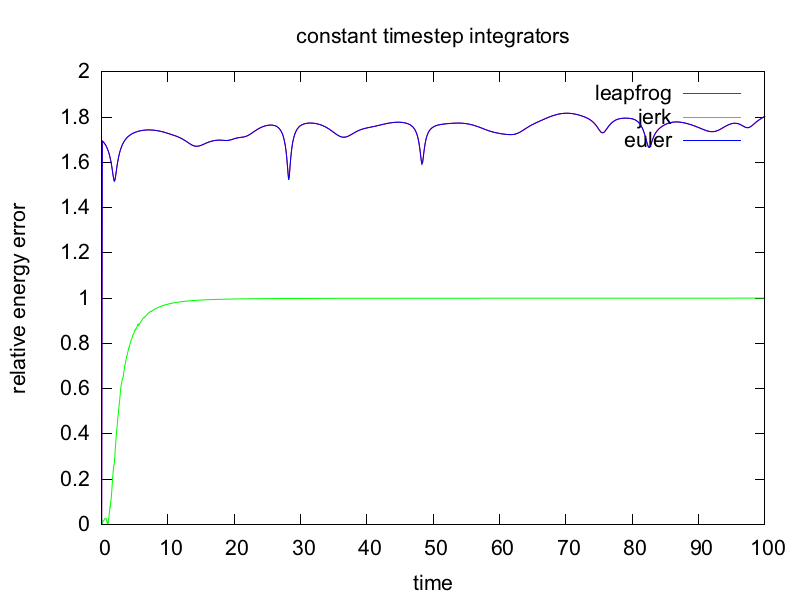
\includegraphics[width=0.9\textwidth]{constant_time.png}
    \caption{Relative energy error for the Euler,Taylor and Leapfrog integrator using fixed time-steps for a fixed total model simulation time.}
    \label{fig:leapfrog}
\end{figure}
However, the Taylor integrator comes with extra costs in computation time as can be seen in figure~\ref{fig:time}. The calculation time for calculating one extra Taylor term, i.e. the jerk, doubles the total computation time. Also, the figure shows that the increase in bodies has a quadratic behavior which is to be expected with $n^2$ complexity in the Euler integrator. 
\begin{figure}
    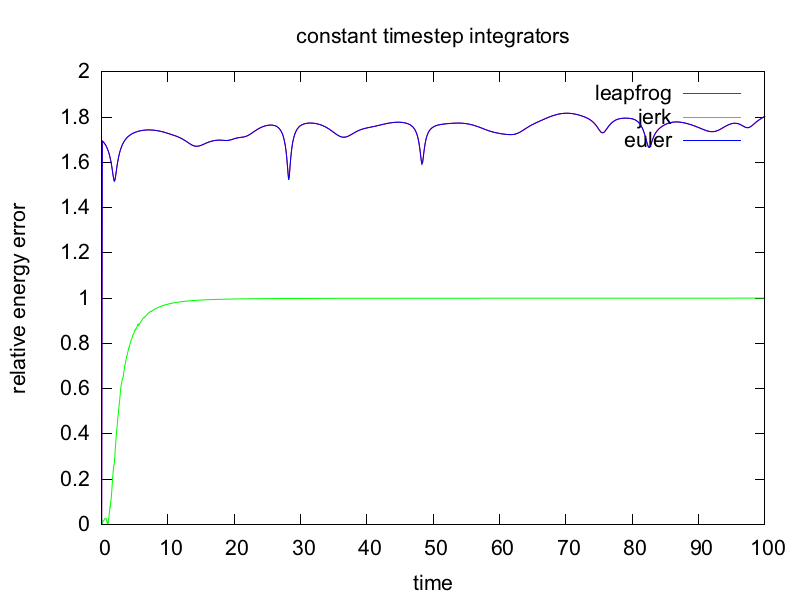
\includegraphics[width=0.9\textwidth]{constant_time.png}
    \caption{Computation time to finish calculating the total model simulation time for a given number of bodies.}
    \label{fig:time}
\end{figure}

\section{Conclusions}
\label{sec:conclusion}
We have simulated different integrators and found a metric to compare the different models with each other. However, there is not one best model to select. Depending on the intentions of the simulation different models might be more applicable. For example, when speed has more priority than accuracy the Euler model might be more appropriate. Nevertheless, this research shows the complex considerations you have to take into account to build a simulation model. Also, that theoretical improvements do not always lead to actual improvements in a computer simulation. 

\section{Future work}




\bibliographystyle{alpha}
\bibliography{article}
\end{document}

